\documentclass[a4paper]{article}
\usepackage[pdftex]{hyperref}
\usepackage[latin1]{inputenc}
\usepackage[english]{babel}
\usepackage{a4wide}
\usepackage{amsmath}
\usepackage{amssymb}
\usepackage{algorithmic}
\usepackage{algorithm}
\usepackage{ifthen}
\usepackage{listings}
% move the asterisk at the right position
\lstset{basicstyle=\ttfamily,tabsize=4,literate={*}{${}^*{}$}1}
%\lstset{language=C,basicstyle=\ttfamily}
\usepackage{moreverb}
\usepackage{palatino}
\usepackage{multicol}
\usepackage{tabularx}
\usepackage{comment}
\usepackage{verbatim}
\usepackage{color}

%% pdflatex?
\newif\ifpdf
\ifx\pdfoutput\undefined
\pdffalse % we are not running PDFLaTeX
\else
\pdfoutput=1 % we are running PDFLaTeX
\pdftrue
\fi
\ifpdf
\usepackage[pdftex]{graphicx}
\else
\usepackage{graphicx}
\fi
\ifpdf
\DeclareGraphicsExtensions{.pdf, .jpg}
\else
\DeclareGraphicsExtensions{.eps, .jpg}
\fi

\parindent=0cm
\parskip=0cm

\setlength{\columnseprule}{0.4pt}
\addtolength{\columnsep}{2pt}

\addtolength{\textheight}{5.5cm}
\addtolength{\topmargin}{-26mm}
\pagestyle{empty}

%%
%% Sheet setup
%% 
\newcommand{\coursename}{Machine Learning}
\newcommand{\courseno}{CO22-320372}
 
\newcommand{\sheettitle}{Homework}
\newcommand{\mytitle}{}
\newcommand{\mytoday}{{May 26th}, 2018}

% Current Assignment number
\newcounter{assignmentno}
\setcounter{assignmentno}{11}

% Current Problem number, should always start at 1
\newcounter{problemno}
\setcounter{problemno}{1}

%%
%% problem and bonus environment
%%
\newcounter{probcalc}
\newcommand{\problem}[2]{
  \pagebreak[2]
  \setcounter{probcalc}{#2}
  ~\\
  {\large \textbf{Problem {\arabic{assignmentno}}.{\arabic{problemno}}} \hspace{0.2cm}\textit{#1}} \refstepcounter{problemno}\vspace{2pt}\\}

\newcommand{\bonus}[2]{
  \pagebreak[2]
  \setcounter{probcalc}{#2}
  ~\\
  {\large \textbf{Bonus Problem \textcolor{blue}{\arabic{assignmentno}}.\textcolor{blue}{\arabic{problemno}}} \hspace{0.2cm}\textit{#1}} \refstepcounter{problemno}\vspace{2pt}\\}

%% some counters  
\newcommand{\assignment}{\arabic{assignmentno}}

%% solution  
\newcommand{\solution}{\pagebreak[2]{\bf Solution:}\\}

%% Hyperref Setup
\hypersetup{pdftitle={Homework \assignment},
  pdfsubject={\coursename},
  pdfauthor={},
  pdfcreator={},
  pdfkeywords={Machine Learning},
  %pdfpagemode={FullScreen},
  %colorlinks=true,
  %bookmarks=true,
  %hyperindex=true,
  bookmarksopen=false,
  bookmarksnumbered=true,
  breaklinks=true,
  %urlcolor=darkblue
  urlbordercolor={0 0 0.7}
}

\begin{document}
\coursename \hfill Course: \courseno\\
Jacobs University Bremen \hfill \mytoday\\
{Zihan Qi \& Danni Long}\hfill
\vspace*{0.3cm}\\
\begin{center}
{\Large \sheettitle{} {\assignment}\\}
\end{center}

\section*{Procedure}
\textbf{Structure:}\\
MLP:
input: 3 units, hidden layer: 3 units, output: 1 units.\\\\
We started with 2 Class, one for hidden layer, one for output layer. Both of them have initial weight matrix size defined based on number of input number, and corresponding initial weight value, forward and back propagation functions. Hidden layer has sigmoid function for wrapping outside potential value from linear combination of activation values of input sample. Output layer has mean square error function, and a threshold function for computing the error between true values and the output of hidden layer after threshold, for further back propagation.\\\\
\textbf{Concrete Implementation:}\\
We have 4 input, each of which has 3 units, first place is a bias term --1. Then based on initialization, now we have a 3$\times$2 matrix, so that linear combination of the every units contributes to 2 units in hidden layer. A sigmoid function was wrap outside the result. Then a bias term was added on top of the 2 units. Based on our initialization of output layer, we have a 3$\times$1 weight matrix, to make linear combination of 3 units from hidden layer for the one output unit in output layer.\\
Now we finished forward pass, and got a result. It is a value in [0,1], then we applied the threshold function to determined it to be \{0,1\}.\\
Afterwards, output of a list of 0/1 will compare with target output, and compute the error. Since there was no sigmoid function when compute output units, we could directly have its partial derivative for gradient descent. Then update second weight matrix from its random initialization. Then for hidden layer, we compute the error from we had in output layer, and update its weight.\\
This whole process is one epoch, and we repeat doing it for 3000 times, in step size 0.1.\\\\
We plot the MSE in Case 1: use values after threshold to compute with target values. It will have spikes, since both of values only have 0/1. Around 2600 epochs, MSE convergent to 0 error.\\
Case 2: direct use output values, compare with target values. (but still use the threshold do back propagation), the error will be more smooth. Since each time output is a continuous value in [0,1]. Around 2600 epochs, the MLP convergent to a small fixed error.\\\\
\begin{figure}[h]
  \centering
    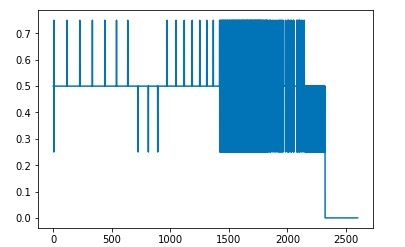
\includegraphics[height = 2.2in]{case1.JPG}
    \caption{Case 1}
\end{figure}
\begin{figure}[h]
  \centering
    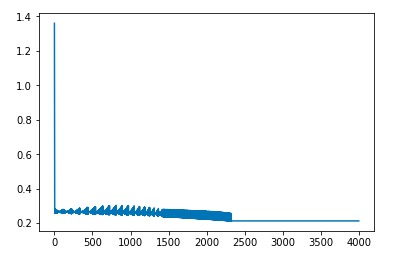
\includegraphics[height = 2.2in]{case2.JPG}
    \caption{Case 2}
\end{figure}
\newpage
\textbf{Bonus:}\\
We picked continuous version of XOR. We change activation function from sigmoid to tahn, since tahn maps value from [-1,1], which coincides with the sign function we are trying to approximate (But sigmoid will still do the work). The network wasn't convergent in the first place, we tune down the learning rate from 0.1 to 0.03, and added an addition unit in hidden layer, after 6000 epoch, the MSE convergence to a bit smaller than 1. We were suspicious about the error, but the output result are correct if you compare to the result from sign function. The reason why errors stay around 1 is what we believe cased by the threshold function we set. When doing back propagation, we let continuous value output which less than 0 to be -1, 0 to be 0 and larger than 0 to be 1. so as soon as the value over 0 a bit, it is recognized as 1, if the true label is 1 then the tuning process will leave this value alone. Therefore, If you look at output printed out, it is a vector of very small value around 0, yet they are correct. Our 2D contour plot has error, so we didn't include it.\\

\begin{figure}[h]
  \centering
    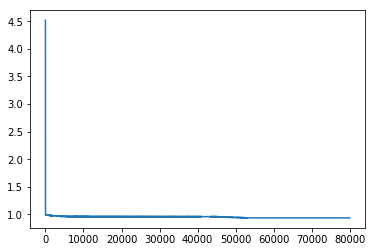
\includegraphics[height = 2.2in]{Bonus.png}
    \caption{Bonus}
\end{figure}
\newpage
Below is the case we choose learning rate to be 0.1, and using 2 units in hidden layer. You may observe that the network was not stable. so we tune down the learning rate, and magnitude is also decreasing.\\
Then we added more units in hidden layer, you could observe the MSE much more faster. In the case of hidden layer has 10 units, MSE convergence with epoch = 600.\\
\begin{figure}[h]
  \centering
    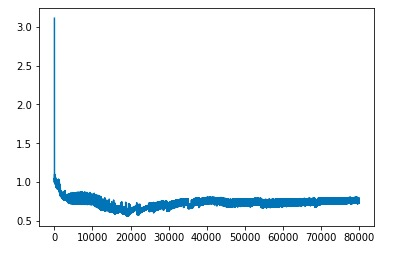
\includegraphics[height = 2.2in]{IMG_1217.JPG}
    \caption{Bonus}
\end{figure}
\begin{figure}[h]
  \centering
    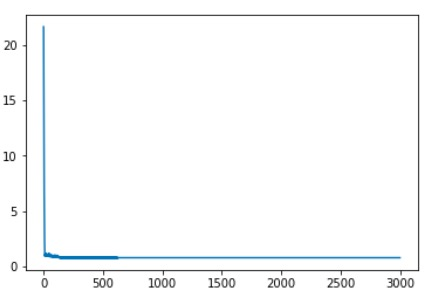
\includegraphics[height = 2.2in]{IMG_1218.JPG}
    \caption{Bonus}
\end{figure}

\end{document}
